%% 
%% Copyright 2007, 2008, 2009 Elsevier Ltd
%% 
%% This file is part of the 'Elsarticle Bundle'.
%% ---------------------------------------------
%% 
%% It may be distributed under the conditions of the LaTeX Project Public
%% License, either version 1.2 of this license or (at your option) any
%% later version.  The latest version of this license is in
%%    http://www.latex-project.org/lppl.txt
%% and version 1.2 or later is part of all distributions of LaTeX
%% version 1999/12/01 or later.
%% 
%% The list of all files belonging to the 'Elsarticle Bundle' is
%% given in the file `manifest.txt'.
%% 
%% Template article for Elsevier's document class `elsarticle'
%% with harvard style bibliographic references
%% SP 2008/03/01

\documentclass[preprint,12pt,authoryear]{elsarticle}

%% Use the option review to obtain double line spacing
%% \documentclass[authoryear,preprint,review,12pt]{elsarticle}

%% Use the options 1p,twocolumn; 3p; 3p,twocolumn; 5p; or 5p,twocolumn
%% for a journal layout:
%% \documentclass[final,1p,times,authoryear]{elsarticle}
%% \documentclass[final,1p,times,twocolumn,authoryear]{elsarticle}
%% \documentclass[final,3p,times,authoryear]{elsarticle}
%% \documentclass[final,3p,times,twocolumn,authoryear]{elsarticle}
%% \documentclass[final,5p,times,authoryear]{elsarticle}
%% \documentclass[final,5p,times,twocolumn,authoryear]{elsarticle}

%% For including figures, graphicx.sty has been loaded in
%% elsarticle.cls. If you prefer to use the old commands
%% please give \usepackage{epsfig}

%% The amssymb package provides various useful mathematical symbols
\usepackage{amssymb}
\usepackage{amsmath}
\usepackage{color, soul}
\usepackage{url}
\usepackage{booktabs}
\usepackage{longtable}
\usepackage{lscape}
%% The amsthm package provides extended theorem environments
%% \usepackage{amsthm}

%% The lineno packages adds line numbers. Start line numbering with
%% \begin{linenumbers}, end it with \end{linenumbers}. Or switch it on
%% for the whole article with \linenumbers.
\usepackage{lineno}

%% Block of code for fixing corresponding author bug 
%% in elsarticle template... Don't really understand it
\makeatletter
\def\@author#1{\g@addto@macro\elsauthors{\normalsize%
    \def\baselinestretch{1}%
    \upshape\authorsep#1\unskip\textsuperscript{%
      \ifx\@fnmark\@empty\else\unskip\sep\@fnmark\let\sep=,\fi
      \ifx\@corref\@empty\else\unskip\sep\@corref\let\sep=,\fi
      }%
    \def\authorsep{\unskip,\space}%
    \global\let\@fnmark\@empty
    \global\let\@corref\@empty  %% Added
    \global\let\sep\@empty}%
    \@eadauthor={#1}
}
\makeatother
%% End block of weird code


%% Command for bold Greek symbols
\newcommand{\mitbf}[1]{\hbox{\mathversion{bold}$#1$}}

\journal{Earth and Planetary Science Letters}

\begin{document}

\begin{frontmatter}

%% Title, authors and addresses

%% use the tnoteref command within \title for footnotes;
%% use the tnotetext command for theassociated footnote;
%% use the fnref command within \author or \address for footnotes;
%% use the fntext command for theassociated footnote;
%% use the corref command within \author for corresponding author footnotes;
%% use the cortext command for theassociated footnote;
%% use the ead command for the email address,
%% and the form \ead[url] for the home page:
%% \title{Title\tnoteref{label1}}
%% \tnotetext[label1]{}
%% \author{Name\corref{cor1}\fnref{label2}}
%% \ead{email address}
%% \ead[url]{home page}
%% \fntext[label2]{}
%% \cortext[cor1]{}
%% \address{Address\fnref{label3}}
%% \fntext[label3]{}

\title{Bayesian inversion for paleomagnetic reconstruction and plate kinematics}

%% use optional labels to link authors explicitly to addresses:
%% \author[label1,label2]{}
%% \address[label1]{}
%% \address[label2]{}

\author{Ian Rose\corref{cor1}\fnref{ref1}}
\author{Bruce Buffett\fnref{ref1}}
\author{Nicholas Swanson-Hysell\fnref{ref1}}

\fntext[ref1]{University of California, Berkeley}
\cortext[cor1]{Corresponding author, \url{ian.rose@berkeley.edu}}

\address{}

\begin{abstract}

\end{abstract}

\begin{keyword}
%% keywords here, in the form: keyword \sep keyword

%% PACS codes here, in the form: \PACS code \sep code

%% MSC codes here, in the form: \MSC code \sep code
%% or \MSC[2008] code \sep code (2000 is the default)

\end{keyword}

\end{frontmatter}

\linenumbers

%% main text
\section{Introduction}
\label{sec:introduction}

Plate tectonics is the motion of near-rigid blocks of lithosphere across the surface of Earth, 
separated by narrow regions of deformation in spreading centers, transform faults, and subduction zones.
The overall rigidity of plate motions means that the motion of a great majority of Earth's surface
can be described by a set of Euler poles which specify the position and magnitude of the rotation axis for a
given plate \citep[cf.][]{cox2009plate}. The motion of individual points on a plate undergoing
a rigid rotation is described by small circles.

Euler poles are ubiquitous in describing current plate motions 
\citep[e.g.][]{demets1990current, argus2011geologically} due to their simplicity and compactness.
Furthermore, there are good reasons to think that plate motions remain constant, or approximately
so, over millions to tens of millions of years. This is most dramatically seen in the shape
of oceanic fracture zones and in hotspot tracks across the lithosphere. These features
form gently curving arcs over large portions of Earth's surface which are well described by small
circles, consistent with finite Euler rotations of the plate for an extended period of time.
As such, the combination of an Euler pole plus a time interval through which it rotates 
(often called a ``stage pole'') is a convenient description of plate motions through Earth history.

The stage pole description of plate motions is therefore a convenient way of reconstructing
plate tectonic history, and is widely used in both continental reconstruction 
\citep[e.g.][]{boyden2011next} and in geodynamical
modeling \citep[e.g.][]{mcnamara2005thermochemical, bull2014effect, rudolph2014history}.
Most reconstructions of plate motions rely heavily on fitting Euler pole rotations
to oceanic fracture zones, hotspot tracks, seafloor magnetic isochrons,
and, to a lesser extent, paleomagnetic data \citep{muller1993revised, seton2012global}.
However, as we look further back in Earth history, the records on which these
plate tectonic reconstructions rely largely disappear due to the continual
subduction of oceanic lithosphere. Before $\sim$200 Ma there is no oceanic record,
and the paleomagnetic record from continental rocks is all that remains.

It is more challenging to reconstruct past plate motions from the paleomagnetic
record for a number of reasons, including 
(1) the data is usually sparser and with larger uncertainties,
(2) traditional paleomagnetic analysis has no way of constraining paleolongitude, and
(3) many paleomagnetic poles have poor age control.

\citet{gordon1984paleomagnetic} noted that apparent polar wander paths (APWPs) have 
arcing trajectories similar to fracture zones and hotspot tracks, which is
to be expected if similar tectonic processes are responsible for creating them.
They therefore suggested fitting small circles to paleomagnetic poles tracks,
which would furnish Euler poles for the plate in question for that time period.
This model for understaning APWPs, called paleomagnetic Euler pole (PEP) analysis,
 had the attractive feature of providing a complete description of the plate motion, 
including paleolongitudinal changes and speeds. 
However, it had the drawback of being somewhat difficult to calculate,
uncertainties in the fit were not easily computed, 
and it did not incorporate age uncertainties. 
A rigorous treatment of the uncertainties requires significant computational effort.
With a few exceptions \citep{beck1989paleomagnetism, tarling1996palaeomagnetic, bryan1986rotation, beck2003absolute, smirnov2010co} 
PEP analysis has not seen wide adoption.

Herein we extend paleomagnetic Euler pole analysis by placing it within
a Bayesian statistical framework, and demonstrate how to invert for PEPs
using Markov Chain Monte Carlo (MCMC) methods. This framework has the advantage
of naturally incorporating uncertainties in the paleomagnetic pole positions,
as well as widely disparate age uncertainties that commonly occur in APWPs.
The resulting stage poles for which we invert is not a single answer, but is instead
a distribution of possible answers, furnishing uncertainties as part of the solution process.

The paper is organized as follows: in Section~\ref{sec:apwp} we review different
approaches for interpreting APWPs. In Section~\ref{sec:bayesian_inversion} we
describe the formalism of Bayesian inversions and Markov Chain Monte Carlo methods.
In Section~\ref{sec:model} we describe the statistical model which we will be inverting.
In Section~\ref{sec:example_inversion} we demonstrate the inversion on several
synthetic data sets. In Sections~\ref{sec:australia} and~\ref{sec:keweenawan}
we show examples using real paleomagnetic data from Australia and Laurentia,
including interpretations of plate speeds.

\section{Interpretation of APW paths}
\label{sec:apwp}
\begin{figure*}
%%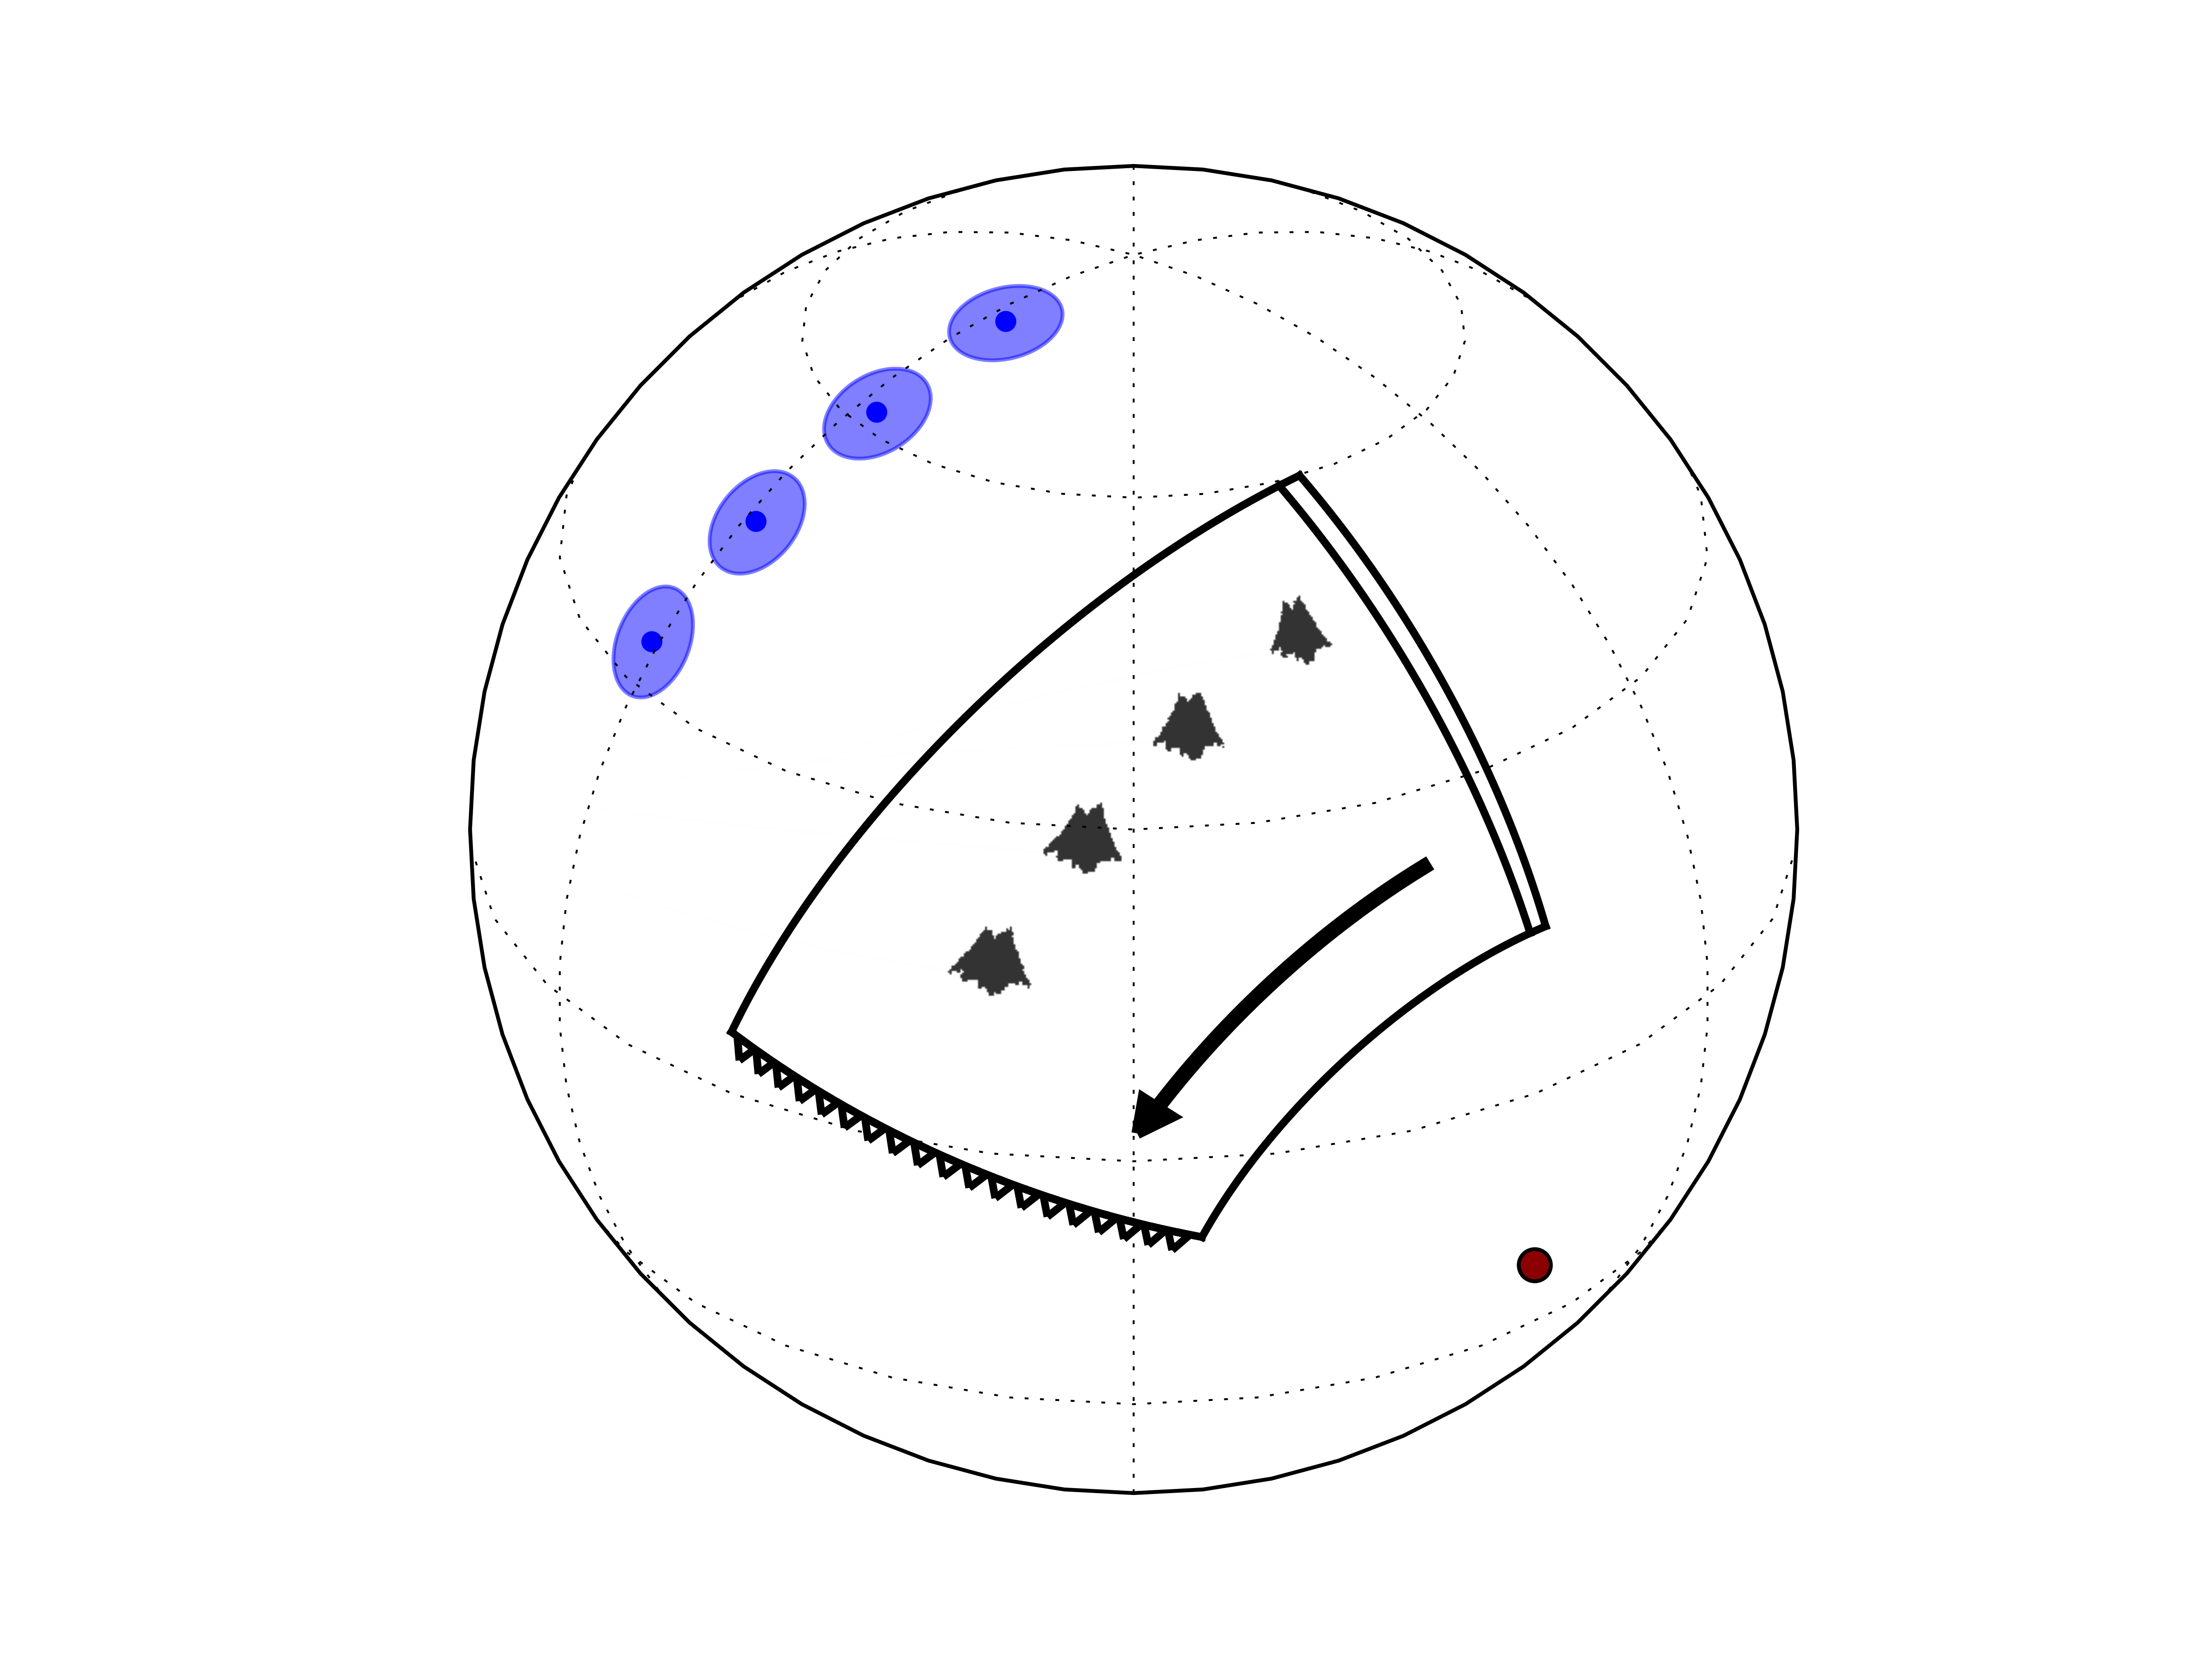
\includegraphics[width=0.9\textwidth]{figures/cartoon/paleomagnetic_euler_pole.png}
\caption[Conceptual model for a paleomagnetic Euler pole.]{Conceptual model for a paleomagnetic Euler pole. A finite rotation of the plate around an Euler pole results in long, arcuate oceanic fracture zones and hotspot tracks which describe small circles on the globe. The same finite rotation produces a small circle in the APW path. By fitting a small circle to the APW path we may recover the Euler pole that produced the rotation.}
\label{fig:pep}
\end{figure*}
A sequence of paleomagnetic poles from the same contintental block form an APW path,
which can then be analyzed to inform plate tectonic reconstructions and dynamic models
of plate speeds through time. Interpretation of these paths becomes difficult in the
case of limited or high-uncertainty data, and when the paleomagnetic poles are of uncertain
ages. A number of approaches to dealing with uncertainty in APW paths have been developed,
which we briefly review here.

\subsection{Latitudinal drift}
Due to the rotational symmetry of Earth's magnetic field, paleomagnetic poles do not
directly constrain the paleolongitude of the continental block in question \citep{butler1992paleomagnetism}.
The simplest analysis of an APW path is thus to compare the paleolatitudes of successive poles.
The difference in paleolatitudes gives a mininimum distance over which the block has traveled, 
corresponding to the great circle path between the two poles. If the two poles are well-dated,
this also furnishes a rate of latitudinal motion.

It is also possible to estimate confidence bounds on the rate of latitudinal drift by
bootstrap resampling \citep[e.g.][]{tarduno1990fast} or by taking a Monte Carlo approach. 
\citet{swanson2014confirmation} generated samples from Fisher distributions
for a pair of poles from the Proterozoic Laurentian midcontinent rift zone to estimate the range
of allowable latitudinal drift rates. They also sampled from the age uncertainties, assuming
Gaussian distributions on the radiometric dates, which incorporated the age uncertainties of the poles.

Whether using point estimates of the latitudinal drift rate or using Monte Carlo estimates, 
the latitudinal drift interpretation of APW paths remains limited.
It has no control over longitudinal drift rate, 
nor does it naturally extend to APW paths with more than two poles, 
especially if two coeval poles are not in agreement.

\subsection{Spherical splines}

When considering APW paths with many poles, it becomes more difficult to perform
latitudinal comparisons between pairs of poles. It is not always clear which pairs of
poles to compare in cases where there are many overlapping paleomagnetic poles,
often of unclear age progression and variable reliabilities.

One approach to deal with these uncertainties is to fit a spline through the
set of paleomagnetic poles, constrained to lie on the surface of a sphere.
This approach was pioneered by \citet{torsvik1992baltica} using the spherical spline
algorithm developed by \citet{jupp1987fitting}.
This approach has the advantage of allowing the weighting of the data by their
uncertainties. The uncertainty assigned to a paleomagnetic pole can
be the 95\% confidence interval on the pole, but it can also be augmented
by various quality screening factors, such as the ``Q'' factor of \citet{van1990reliability} \citep{torsvik1992baltica}. 
Even with the weighting of the paleomagnetic poles by uncertainty there
can be unrealistic loops in the APW path generated by the spline fit.
To combat this, the spline can also be computed under tension, penalizing
curvature and producing a smoother path \citep{torsvik1996continental}.

The spherical spline approach to interpreting APW paths has several attractive features.
It produces a smooth path through the data, incorporates spatial uncertainties
in the data, and may be efficiently computed.
However, it does have some drawbacks.
It is not easy to determine the appropriate uncertainty weighting and spline
tension parameters for the fit, and what effect those choices have on the result.
Furthermore, the resulting fit does not have an uncertainty with a physically
interpretable meaning \citep{torsvik1996continental}.
It also does not have a simple way of incorporating age uncertainties of the paleomagnetic poles.
Finally, by their very nature, splines cannot represent the sharp hairpin cusps
that characterize the abrupt shifts in motion that plates undergo \citep{irving1972hairpins, gordon1984paleomagnetic}.

\subsection{Running means}

An alternative method for smoothing APW paths is to perform a running Fisher
mean on the poles with a moving window \citep{van2001evidence, torsvik2008global}.
Typically the observed paleomagnetic poles are averaged every 1-10 Myr with a 10-30 Myr
window size. Like spherical splines, the running mean approach has the ability
to effectively damp spurious loops in the APW path, with the width
of the moving window controlling the amount of smoothing.
Furthermore, it enforces an age progression in the averaged poles.
\citet{torsvik2008global} also investigated the effects of combining running means
with spherical splines, by first computing a set of mean poles and then
fitting a spline through those means.

Unfortunately, the running mean approach shares many of the drawbacks of the spline approach. 
It is not obvious how to best choose the window size, 
and it is not clear how to interpret the resulting uncertainties in the path.
It, too, does not easily incorporate age uncertainties in the poles.

\subsection{Paleomagnetic Euler poles}

Paleomagnetic Euler poles (PEP, introduced in Section~\ref{sec:introduction}, 
also known as the ``small circle'' method, were first described by \citet{gordon1984paleomagnetic}.
The model rests in recognizing that plate motions are well described by finite
rotations around Euler poles which are approximately steady for millions or 
tens of millions of years. A result of this is that the apparent polar
wander path of the plate can be described by the same rotations, which
produce small circles on Earth's surface.

By fitting a sequence of Euler poles to a small circle path, one specifies
the position of the Euler pole which produces that circle.
PEP analysis has the feature that it closely hews to our model for how plates move.
Since it specifies the Euler pole which produces a given small circle,
this allows for an estimate of the longitudinal motion of a given plate, 
as well as the total plate speed (instead of just the latitudinal component of the speed).

On the other hand, Paleomagnetic Euler pole analysis has many of the same
deficiencies that spline fits and running means have: it is not easy to compute
uncertainties, especially in the presence of unknown ages of poles.
Furthermore, one has the additional challenge of deciding how many PEPs to invert.
In the following sections we develop a Bayesian statistical approach to
PEP analysis which attempts to address these deficiencies.

\section{Bayesian inversion}
\label{sec:bayesian_inversion}
\subsection{A general desciption of inverse problems}
\label{sec:intro_inverse_problems}
The central question motivating inverse problems is ``How probable is a particular model, given my observations?''.
We represent a vector of individual observation by the data vector $\mathbf{d}$, and a model
by the vector of model parameters $\mathbf{m}$, so the above question can be written expressed as the function $P(\mathbf{m} \vert \mathbf{d})$.
Traditional frequentist approaches to an inverse problem often proceed by maximizing the likelihood function,
defined by the probability of the data given a particular model:
\begin{equation}
\mathcal{L} ( \mathbf{m} \vert \mathbf{d} ) = P( \mathbf{d} \vert \mathbf{m} ).
\label{eq:likelihood}
\end{equation}
The likelihood function replaces something that is difficult to compute (namely, $P(\mathbf{m} \vert \mathbf{d})$)
with something that is less difficult to compute. 
To compute $\mathcal{L}(\mathbf{m}, \mathbf{d})$ we need to have two things: a statistical model for 
uncertainties in the observations $\mathbf{d}$ and forward model that allows us to compute
predictions ($\mathbf{d}_p$ of the observations from the model parameters, denoted by $\mathbf{g}$:
\begin{equation}
\mathbf{d}_p = \mathbf{g}(\mathbf{m}).
\label{eq:forward}
\end{equation}
For example, if each of the observed data $d_i$ are described with Gaussian uncertainties
with standard deviations $\sigma_i$, the likelihood function is given by the product
of the individual likelihoods of the observations:
\begin{equation}
\mathcal{L}(\mathbf{d} | \mathbf{m} ) = \displaystyle\prod_i \exp\left({-\frac{(d_i - d_{p,i})^2}{2 \sigma_i^2}}\right)
\label{eq:example_likelihood}
\end{equation}
The likelihood function $\mathcal{L}$ is maximized by searching over the model parameter space.
If the uncertainties in the observations are Gaussian, then maximizing the likelihood function is
equivalent to the least squares solution \citep{aster2005parameter}.

Frequently an unomdified maximum likelihood fit will overfit the observations, resulting
in unrealistic solutions. In the context of APW paths, these overfit solutions may
pass through every paleomagnetic pole, including less reliable ones, resulting in
loopy, sinuous paths. In order to address this, some form of regularization is usually
included in the solution of the inverse problem, such as penalizing the magnitude or
curvature of the solution. Both the running-mean and the spline under tension approaches
to APW paths can be seen as a form of regularization on the problem.

\subsection{Bayesian approach}

The Bayesian approach to inverse problems takes a different strategy from the frequentist one.
Rather than finding point estimates of a model fit, it treats the underlying model
as a set of random variables with individual probability distributions.
The probability distribution of the model $P(\mathbf{m} \vert \mathbf{d})$ 
is then found by an application of Bayes theorem \citep[cf.][]{sivia2006data}:
\begin{equation}
P\left(\mathbf{m} \vert \mathbf{d} \right) = \frac{ P \left(\mathbf{d}\vert \mathbf{m} \right) P \left( \mathbf{m} \right) }{P \left( \mathbf{d}\right)}
\label{eq:bayes}
\end{equation}
It is often unnecessary to calculate the denominator of Equation~\eqref{eq:bayes}, leaving
\begin{equation}
P\left(\mathbf{m} \vert \mathbf{d} \right) \propto P \left( \mathbf{d} \vert \mathbf{m} \right) P \left( \mathbf{m} \right) 
\label{eq:propbayes}
\end{equation}
The quantity $P(\mathbf{m} \vert \mathbf{d})$ is known as the posterior probability,
and represents our desired knowledge about the distributions of the paramters $\mathbf{m}$.
The first factor on the left-hand-side of Equation~\eqref{eq:propbayes} is identical to the likelihood
function described in Section~\ref{sec:intro_inverse_problems}, and the second factor
is known as the prior probability.

The prior probability reflects the state of our knowledge and beliefs of the values
of the model parameters prior to the consideration of our data, and can allow us
to incoroporate constraints that are not otherwise included in the forward model.
In contrast with the classical statistical approach of regularization, the Bayesian
inverse problem can (in effect) regularize the problem through the choice of prior, by making
choices of probability distributions that are lower for less realistic values 
\citep{minson2013bayesian, sambridge2013transdimensional}.

\subsection{Markov chain Monte Carlo methods}

It is usually impossible to calculate the posterior
probability distribution in Equation~\eqref{eq:bayes} directly \citep{davidson2015bayesian}. 
It is much more tractable to generate a Markov chain which, in the long run,
generates samples from the desired posterior \citep{gelman2014bayesian}, a
class of methods known as Markov chain Monte Carlo (MCMC) methods.

The literature on MCMC methods is extensive and we do not cover it here, but
the interested reader can refer to \citet{gelman1996markov}, \citet{sambridge2013transdimensional},
and \citet{davidson2015bayesian}. A number of high-quality free software packages
for implementing MCMC models exist, including WinBUGS \citep{lunn2000winbugs}, 
PyMC \citep{patil2010pymc}, and Stan \citep{carpenter2016stan}.
In this work we make extensive use of PyMC.

\subsection{Distributions on a sphere}

In order to proceed with a Bayesian description of the problem, every parameter
in the model should be described by some statistical distribution that determines
the probability that the parameter takes a specific value.
Parameters like pole ages can be described by familiar 1D probability distributions
(such as uniform or normal distributions), whereas Euler pole locations are
described by 2D distributions on the surface of a sphere.
We review several of these distributions here.
For a comprehensive discussion of spherical probability distributions,
see \citet{fisher1987statistical}. Plots of the following distributions, as well as
samples drawn from them, are shown in Figure~\ref{fig:distributions}. 


\subsubsection{Uniform distribution}
\begin{figure*}
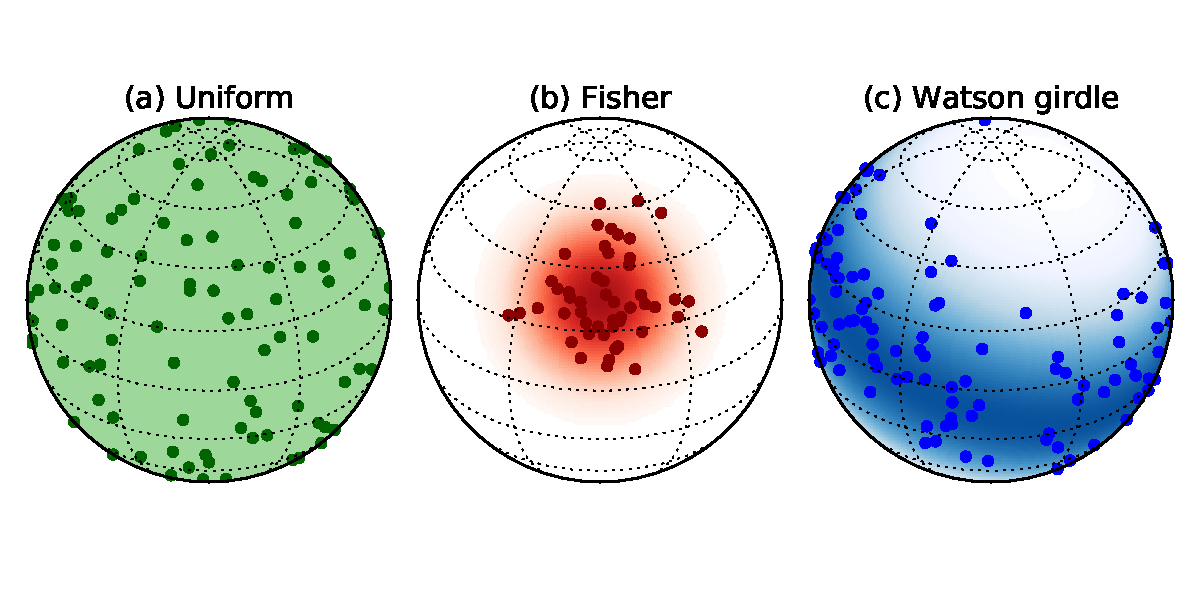
\includegraphics[width=0.9\textwidth]{figures/cartoon/distributions.pdf}
\caption[Spherical probability distributions.]{Probability densities for spherical distributions, as well as samples drawn from them. All are plotted using an orthographic projection. (a) Uniform distribution. (b) Fisher distribution. The center of the distribution is at $30^\circ$N, $30^\circ$E, and the concentration parameter $\kappa=20$. (c) Watson girdle distribution. The pole of symmetry is at $70^\circ$N, $90^\circ$E, and the concentration parameter $\kappa=-5$.}
\label{fig:distributions}
\end{figure*}

The simplest probability distribution on a sphere is the spherical uniform distribution.
It has a probability density given by
\begin{equation}
  \rho_U(\phi, \psi) = \frac{1}{4 \pi},
\end{equation}
where $\rho_U$ is the probability density, $\phi$ is the longitude, and $\psi$ is the latitude.
Most non-uniform distributions on a sphere reduce to the uniform distribution in some limit.
We will use this distribution when we want to specify an uninformative prior for directional parameters.

\subsubsection{Fisher distribution}
The Fisher distribution (also called the von Mises-Fisher distribution) is the analogue
of a 2D normal distribution on a sphere.
The probability density $\rho_F$ for a unit vector $\hat{\mathbf{x}}$ is given by
\begin{equation}
  \begin{aligned}
  \rho_F(\phi, \psi ; \kappa_F, \hat{\mitbf{\mu}}) 
  &= \frac{1}{C_F} \exp \left( \kappa_F \hat{\mathbf{x}}^T \hat{\mitbf{\mu}} \right) \\
  &= \frac{1}{C_F} \exp \left( \kappa_F \cos \theta \right),
  \end{aligned}
\end{equation}
where $\kappa_F$ is the concentration of the distribution, 
$\hat{\mitbf{\mu}}$ the unit vector of the pole of the distribution, 
and $C_F$ is a normalization coefficient. It can be alternatively
parameterized using $\theta$, which is the angle between $\hat{\mathbf{x}}$ and $\hat{\mitbf{\mu}}$.
The normalization factor is given by 
\begin{equation}
  C_F = \frac{\kappa_F}{4 \pi \sinh{\kappa}}.
\end{equation}
When $\kappa_F$ goes to zero, the Fisher distribution is equivalent to the spherical uniform distribution.

The position and uncertainty of most paleomagnetic poles are represented by Fisher distributions,
and so we will use it to calculate the likelihood function of the model.

\subsubsection{Watson girdle distribution}
Whereas the Fisher distribution concentrates probability density near around a pole on
the surface of the sphere, the Watson girdle probability distribution is concentrated
in a belt orthogonal to the pole. It is useful for characterizing planar data, and is given by
\begin{equation}
  \begin{aligned}
  \rho_W(\phi, \psi; \kappa_W, \hat{\mitbf{\mu}}) 
  &= \frac{1}{C_W} \exp \left( \kappa_W (\hat{\mathbf{x}}^T \hat{\mitbf{\mu}})^2 \right) \\
  &= \frac{1}{C_W} \exp \left( \kappa_W \cos^2 \theta \right)
  \end{aligned}
\label{eq:watson}
\end{equation}
where $\kappa_W$ is the concentration of the girdle, $C_W$ is a normalization coefficient,
and the other parameters are identical to those in the Fisher distribution.
The Watson distribution is girdle-shaped only when $\kappa_W$ is a negative number, 
which is the only case we consider here.
The normalization factor is given by
\begin{equation}
  C_W = \left[ {}_1 F_1 \left( \frac{1}{2}, \frac{3}{2}, \kappa_W \right) \right]^{-1}
\end{equation}
where ${}_1 F_1()$ is Kummer's confluent hypergeometric function, which is available
in most software libraries of special mathematical functions.
As with the Fisher distribution, when $\kappa_W$ goes to zero, 
the Watson distribution is equivalent to the spherical uniform distribution.

\section{A model for PEP inversion}
\label{sec:model}
\subsection{Forward model}
\label{sec:forward_model}
The forward model for PEP analysis is essentially unchanged from that of \citet{gordon1984paleomagnetic}.
We describe plate motions (and hence paleomagnetic pole motions) with a series of Euler poles.
Each Euler pole has three parameters for which we are inverting (a latitude, a longitude, and a rotation rate).

We furthermore need to specify the ages where we transition from 
one Euler pole to the next (the cusps, or ``hairpins'' of \citet{irving1972hairpins}).
In the context of parameter inversion these are often known as ``changepoints.''

Finally, we need a starting position on the globe, which, in practice, can be sampled
from the Fisher distribution of the oldest paleomagnetic pole in the dataset.
The starting point contributes two parameters (a latitude and a longitude).

All together, this means that for an inversion with $n_e$ Euler poles, 
we have $3 n_e$ parameters for the poles, $(n_e-1)$ parameters for the changepoints,
and 2 parameters for the starting location.
The number parameters for which we are inverting is then given by
\begin{equation}
\begin{aligned}
N &= 3 n_e + (n_e -1) + 2 \\
 &= 4 n_e + 1
\end{aligned}
\label{eq:n_parameters}
\end{equation}

For each Euler pole $\mitbf{\omega}_i$ the velocity $\mathbf{v}$ of a point 
$\mathbf{p}$ on the surface of the globe is given by
\begin{equation}
\mathbf{v} = \mitbf{\omega}_i \times \mathbf{p}.
\label{eq:rigid_rotation}
\end{equation}
Finite rotations can be performed by constructing Euler angle rotation matrices \citep[cf.][]{goldstein1965classical}. 
We generate synthetic paleomagnetic pole positions from the forward model by stringing together
finite rotations through the stage poles until the age of the paleomagnetic pole
is reached. These positions can then be compared to the actual paleomagnetic poles in our dataset.

\subsection{Choice of priors}
\label{sec:priors}

Bayesian analysis requires us to specify prior distributions for each of the parameters going into the inverse problem.
These distributions reflect our state of belief about the values of the parameters before we begin,
and allow us the option of incorporating information otherwise not captured by the model.
Frequently we want to avoid biasing the results of the model towards a specific posterior distribution,
so we try to choose as uninformative a prior as possible. Depending upon the context, and the type
of parameter, that choice may vary.
The central parameters in the paleomagnetic Euler pole problem are the Euler pole positions,
the Euler pole magnitudes, the changepoints, the starting point, and the paleomagnetic pole ages, which we treat in turn.

\textbf{Euler pole directions:} 
The first parameter we consider is the position of the Euler poles, which should be drawn
from a spherical probability distribution.
The least informative prior for the i'th Euler pole is the uniform spherical distribution:
\begin{equation}
\hat{\mitbf{\omega}}_i \sim \rho_U(\phi, \psi)
\end{equation}
essentially allowing the Euler pole to be anywhere on the globe with equal probability.

An interesting alternative choice is to inform our prior for Euler pole position based
on current plate motions. It has long been observed that, to first order, plate motions
are well explained by slab-pull torques acting along subduction zones, and to a lesser
extent, ridge push and continental keel effects \citep{forsyth1975relative, gordon1978absolute, richardson1992ridge}.
This observation is explained by the fact that plate tectonics is the 
surface expression of Earth's convection.

We can then ask the question of whether the Euler pole for a given plate is more likely
to be on top of the plate (corresponding to a spinning motion for that plate) or far away
from that plate (corresponding to motion across the surface of Earth).
Given the convective interpretation of plates, we can hypothesize that the second possibility
is more likely (a spinning plate does not participate much in convection \citep{forte1987plate, gable1991convection}).

To test this, we generated position samples on the surface of Earth and computed
the angular distance between that point and the Euler pole for the plate in which that point resides.
We used the NNR-MORVEL56 model for current plate motions \cite{argus2011geologically}
and restricted our analysis to the fourteen largest plates.
We then fit those angular distance samples to a Watson girdle distribution (Equation~\eqref{eq:watson}), 
inverting for the concentration parameter $\kappa_W$.
We find that the distribution is best fit with $\kappa_W \approx -0.8$, which corresponds
to the Euler pole probability density being roughly twice as large $90^\circ$
away from a given point than on top of the point.

\textbf{Euler pole magnitudes:} 
The magnitude of each Euler pole is a strictly positive number, specifying the
rotation rate of that pole (negative rotations can be accomplished by flipping an Euler
pole to the antipode).
There are several possibilities for the prior on the rates.
In order to not bias the inversion towards a particular
rate we can choose a uniform prior with large support:
\begin{equation}
\vert \mitbf{\omega}_i \vert \sim U(0, 4)
\end{equation}
where $U(\cdot, \cdot)$ is a uniform distribution between two values, and is given
in degrees per Myr. Typical rotation rates for present day plate motions
are under $1^\circ$/Myr \citep{argus2011geologically}, which corresponds to rates
of about $13^\circ$/Myr at a position $90^\circ$ from the pole.

Another option is to choose a weakly informative prior for the Euler pole magnitudes
informed by recent plate motions (similar to the Watson girdle prior for the directions).
\citet{zahirovic2015tectonic} found based on Cenozoic and Mesozoic plate reconstructions
that plate speeds much higher than 15 cm/yr were unlikely.
A reasonable choice of distribution for strictly positive numbers is the exponential distribution,
given by
\begin{equation}
\rho_E(x) = \lambda \exp(-\lambda t),
\end{equation}
which has higher probability density at lower values, and falls off exponentially.
We sampled the current plate rates on Earth's surface according to NNR-MORVEL56
and fit those to an exponential distribution. The best fitting scale parameter $\lambda$
for current plate rates is $\lambda\approx2$.
Making this choice of prior for Euler pole rotation rates can bee seen as a form
of regularization on plate speeds.

\begin{figure*}
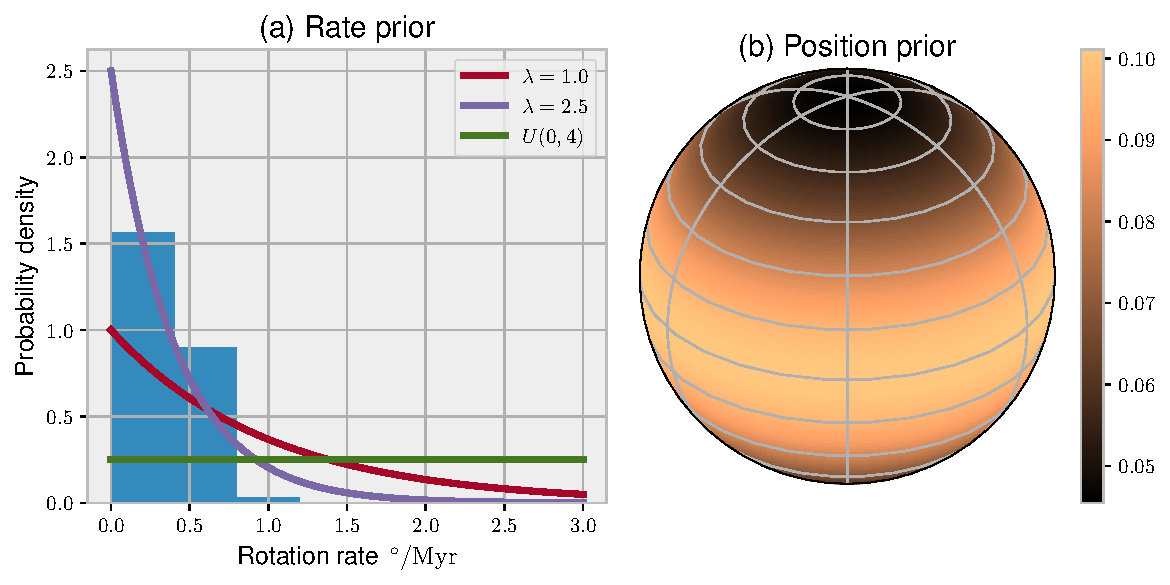
\includegraphics[width=0.9\textwidth]{figures/euler_pole_prior/euler_pole_prior.pdf}
\caption[Informative priors on Euler poles]{Informative priors for Euler poles. (a) Prior probabilities for rotation rates. The histogram is the angular rotation rate from one thousand samples from the surface of Earth, using the NNR-MORVEL56 model. A fit to this sample set with an exponential distribution obtains a scale parameter of $\lambda \approx 2.5$. We also show the distribution for $lambda = 1.0$, which imposes less regularization on the rate. (b) Prior probability density for the position of the Euler poles. We again sampled one thousand points on Earth's surface, calculating the angular distance between that point and the Euler pole for its plate. Fitting the resulting angular distribution to a Watson girdle distribution finds $\kappa_W \approx -0.8$. This results in a probability density roughly twice as large at the equator as at the pole.}
\label{fig:one_euler_pole}
\end{figure*}

\textbf{Changepoints:} 
Changepoints occur sequentially between the oldest (at age $a_\mathrm{max}$) and
youngest (at age $a_\mathrm{min}$) paleomagnetic poles.
We choose a uniform distribution as a prior for these changepoints:
\begin{equation}
c_i \sim U( a_\mathrm{min}, a_\mathrm{max}),
\end{equation}
where $c_i$ is the i'th changepoint.

\textbf{Starting position:}
Finally, the starting position $\hat{\mathbf{x}}_\mathrm{start}$ for the set of Euler pole rotations needs a prior.
We could choose another uniform distribution, but a more reasonable choice
is to start from near the oldest paleomagnetic pole in the dataset.
We therefore choose the Fisher distribution of the oldest paleomagnetic pole as a reasonable prior for a start point:
\begin{equation}
\hat{\mathbf{x}}_\mathrm{start} \sim \rho_F(\phi, \psi; \kappa_{F0}, \hat{\mitbf{\mu_0}})
\end{equation}
where $\kappa_{F0}$ and $\hat{\mitbf{\mu}}_0$ are the concentration parameter and mean direction
of the oldest paleomagnetic pole in the dataset.

\textbf{Pole ages:}
One of the major advantages of Bayesian analysis is the ability to naturally incorporate
uncertainties in as many parameters as we need. Previous approaches to
modeling APWPs have the drawback that they do not easily account for uncertainties in
the age of paleomagnetic poles. In our approach we can include age uncertainty
by simply including the age of the poles as parameters in our model.

There are many different ways to constrain the ages of the geologic units from
which we obtain paleomagnetic poles, including radiometric dating, biostratigraphy,
magnetostratigraphy, cross-cutting relations, and stratigraphic relations.
Here we concentrate on just radiometric dating and stratigraphic constraints.
If a geologic unit has been radiometrically dated, we can model the age of
the j'th paleomagnetic pole $a_j$ as a normal distribution with mean $\mu_j$ and standard deviation $\sigma_j$:
\begin{equation}
a_j \sim N(\mu_j, \sigma_j)
\end{equation}
where $N(.,.)$ denotes a normal distribution.

Freqently, however, the geologic unit from which we obtain a paleomagnetic pole
is not well dated, and its age can only be constrained to lie between those
of well-dated units stratigraphically above and below it. In this case,
we argue that a uniform distribution between those ages is a reasonable choice
of prior:
\begin{equation}
a_j \sim U(a_\mathrm{low}, a_\mathrm{high})
\end{equation}
where $a_\mathrm{low}$ and $a_\mathrm{high}$ are the ages of the upper and lower
well-dated stratigraphic units, respectively.

To summarize our choices for priors:
\begin{itemize}
\item Euler pole positions: spherical uniform distribution, or a Watson girdle distribution with $\kappa_W \approx -0.8$.
\item Euler pole magnitudes: Uniform distribution between 0$^\circ$ and 4$^\circ$/Myr, or an exponential distribution with $\lambda \approx 2$.
\item Changepoints: uniform distribution between $a_\mathrm{min}$ and $a_\mathrm{max}$.
\item Paleomagnetic pole ages: normal or uniform distribution, depending on the type of age control for the geologic unit.
\end{itemize}


\subsection{Likelihood}
\label{sec:likelihood}
In addition to the choice of priors we need a statistical description of the observations.
This will allow us to calculate the likelihood function, which, when combined with the priors,
allows us to evaluate Bayes' theorem (Equation~\eqref{eq:propbayes}).

In the case of APW paths, our observations are paleomagnetic poles.
The most common statistical distribution for describing paleomagnetic poles is the Fisher distribution
(though others are possible, such as the Kent or Bingham distribitions, c.f. \citet{tauxe2009essentials}).
Given the set of model parameters $\mathbf{m}$ and the forward model $\mathbf{g}(\mathbf{m})$, described
in Section~\ref{sec:forward_model}, we can calculate the predicted paleomagnetic pole unit vectors $\hat{\mathbf{x}}_{p,i}$.
For a set of $i$ paleomagnetic poles, the likelihood is then given by the product of the probabilities
of each observation:
\begin{equation}
P(\mathbf{d} \vert \mathbf{m}) = \displaystyle\prod_i \frac{1}{C_{F,i}} \exp \left( \kappa_{F,i} \hat{\mathbf{x}}_{p,i}^T \hat{\mitbf{\mu}}_i \right).
\label{eq:model_likelihood}
\end{equation}


\subsection{Model selection}

\section{Example inversions}
\label{sec:example_inversion}

Before proceeding with inversions for paleomagnetic Euler poles using real paleomagnetic data,
it is useful to consider a few examples of inversions for synthetic datasets.
We have implemented the forward model described in Section~\ref{sec:forward_model}
in Python, and used the package PyMC \citep{patil2010pymc} for performing the Monte Carlo inversion.
We use a Metropolis-Hastings sampler, starting from a fit to the maximum a posteriori (MAP) probability.
In most cases shown here we generate $10^6$ samples, discarding the first 20\%.

\subsection{One stage pole}
\label{sec:one_stage_pole}
We begin by trying to recover the Euler pole for a single rotation.
We generate a synthetic APW track of four poles by starting from a pole at $\phi=30, \psi=0$,
then rotate it around an Euler pole at $\phi=0, \psi=0$ for 180 Myr at $1^\circ$/Myr.
We produce paleomagnetics pole at 190 Ma, 130 Ma, 70 Ma, and 10 Ma, each with an $\alpha_{95}$
of $10^\circ$.

The results are shown in Figure~\ref{fig:one_euler_pole}.
The inversion successfully recovers a posterior probability distribution for the position
of the Euler pole that includes the start pole, as well as a rate that is centered
near the true value of $1^\circ$/Myr. The posterior distribution for the rate
has a highest posterior density (HPD) credible interval at 95\%
between $0.8^\circ$/Myr and $1.2^\circ$/Myr, reflecting the resolving power of the inversion.

\begin{figure*}
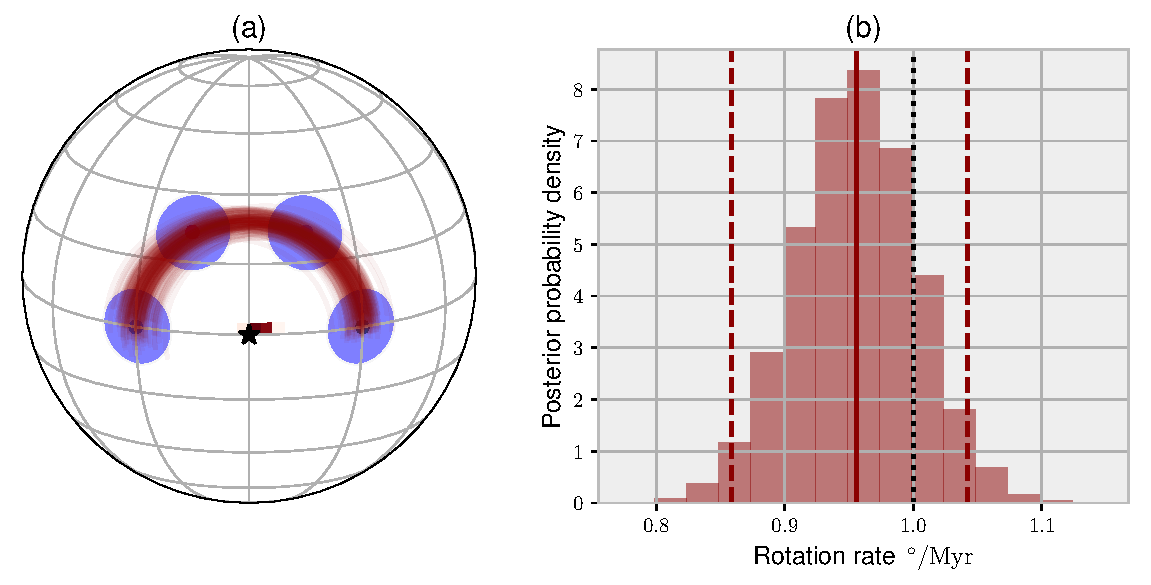
\includegraphics[width=0.9\textwidth]{figures/synthetic/one_euler_pole.pdf}
\caption[Inversion for a single paleomagnetic Euler pole.]{Inversion for a single paleomagnetic Euler pole. (a) Four paleomagnetic poles are generated during a net $180^\circ$ rotation about an Euler pole at $0^\circ$N, $0^\circ$E over 180 Myr, for a rotation rate of $1^\circ$/Myr. The red distribution is the probability density function recovered by MCMC inversion, and the red lines are a sampling of the synthetic APW paths generated by the inversion. (b) Posterior probability density for the rotation rate of the Euler pole recovered by the inversion. The solid line shows the median of the distribution, and the dashed lines show the highest posterior density credible interval at 95\%. }
\label{fig:one_euler_pole}
\end{figure*}

\subsection{Two stage poles}
\label{sec:two_stage_poles}
\begin{figure*}
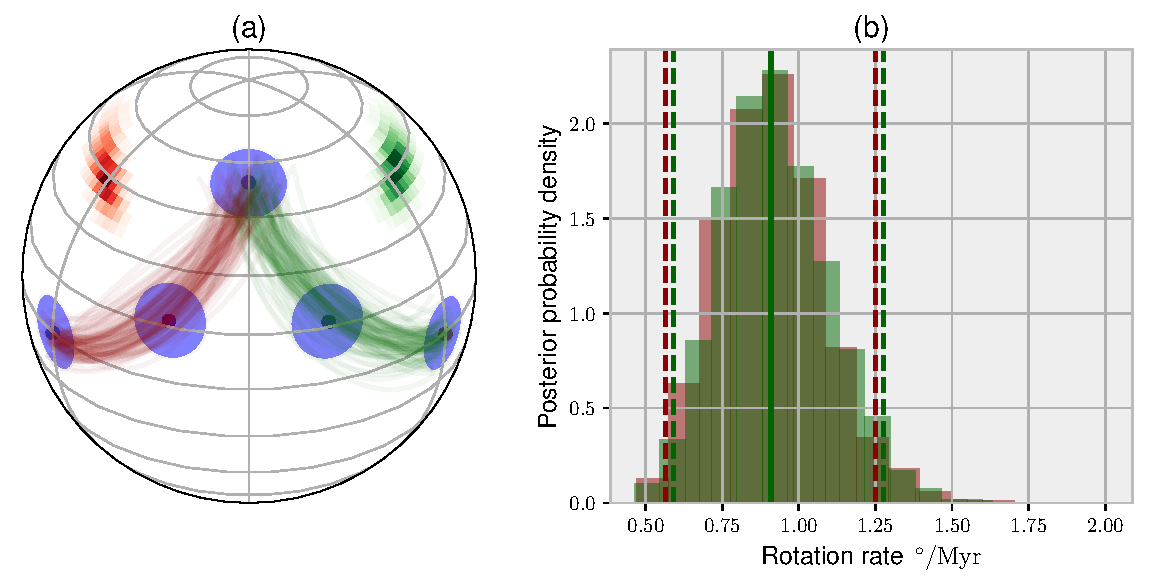
\includegraphics[width=0.9\textwidth]{figures/synthetic/two_euler_poles.pdf}
\caption[Inversion for two successive paleomagnetic Euler poles.]{Inversion for two successive paleomagnetic Euler poles. (a) Five paleomagnetic poles are generated, beginning with a pole at $0^\circ$N, $60^\circ$W. The first Euler pole is located at $41^\circ$N, $60^\circ$W, and rotates at $1^\circ$/Myr for 130 Myr. The second Euler pole is located at $41^\circ$N, $60^\circ$E, and rotates at the same speed and for the same duration. The red and green distributions show the location of the first and second Euler poles (respectively) recovered by the MCMC inversion. The the red and green lines are a sampling of the synthetic APW paths generated by the inversion. (b) Posterior probability density for the rotation rates of the Euler poles recovered by the inversion. The solid lines show the median values of the distributions, and the dashed lines show the HPD intervals. The two distributions are nearly identical, and centered on the true value of the rate.}
\label{fig:two_euler_poles}
\end{figure*}


\subsection{Incorporating age uncertainty}
\label{sec:age_uncertainty}
A major benefit of the Bayesian approach to inverse problems is its great generality.
As long as some effect can be described statistically and incorporated into our
forward model, we can include it in the inverse problem.

In this case, we include uncertainties in the ages of the paleomagnetic poles.
We use the same test case as in Section~\ref{sec:one_stage_pole}, but assign uncertain prior
distributions to the ages of the poles. For the first and last poles we assume they
are radiometrically dated with standard deviations of 2 Myr.
However, we assume that the middle two poles have no age control, except that their
respective rock units lie stratigraphically between the first and last poles.
We thus assign Gaussian priors to the first and last poles and uniform priors
to the middle two.

The primary effect of adding uncertainties to the ages of the poles is that they can
help to constrain the location of the APW path without providing an unwanted constraint
on the timing of the path.
Figure~\ref{fig:age_uncertainty_samples} shows the prior and posterior distributions for the
ages of the poles. We can see from the posterior distribution that the inversion
successfully places the ages of the middle two poles at $\sim70$ Ma and $\sim130$ Ma,
though with relatively wide HPD intervals.
The posterior distributions for the Euler pole position and magnitude 
which we recover from this inversion are visually identical to those in Figure~\ref{fig:one_euler_pole}.

\begin{figure*}
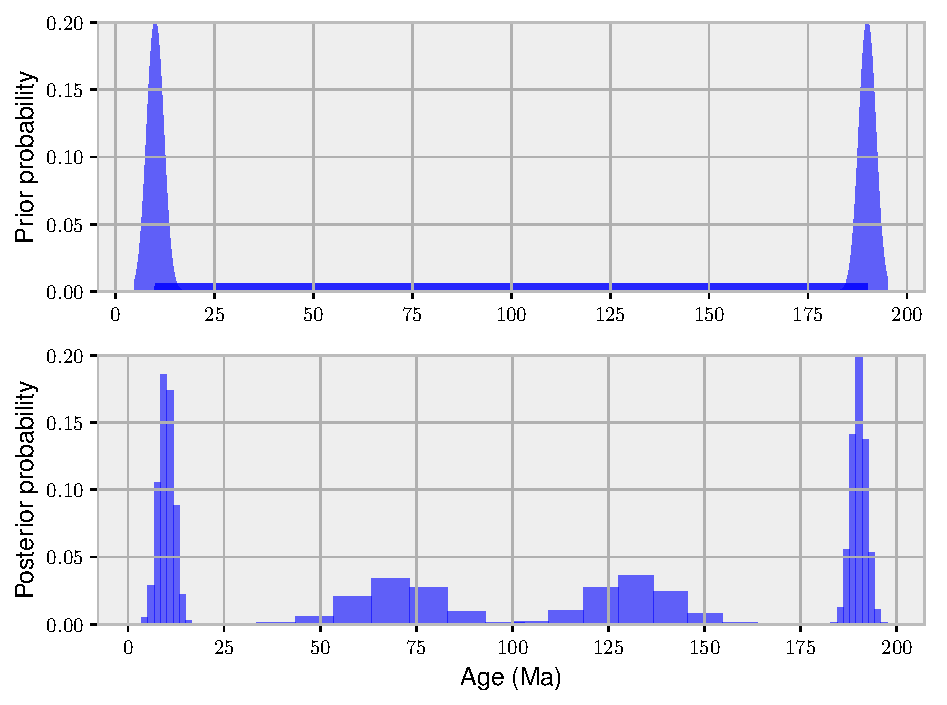
\includegraphics[width=0.9\textwidth]{figures/synthetic/age_uncertainty_samples.pdf}
\caption{}
\label{fig:age_uncertainty_samples}
\end{figure*}

\section{Application to Cenozoic Australian APW path}
\label{sec:australia}
\clearpage
\begin{figure*}
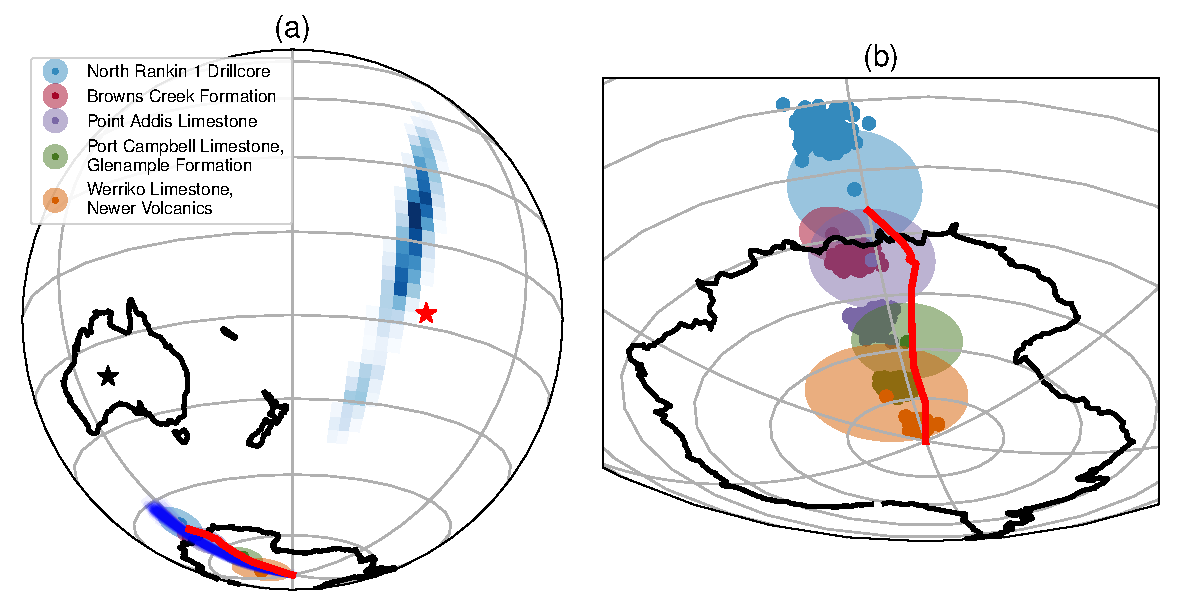
\includegraphics[width=0.9\textwidth]{figures/australia/australia_paths_1.pdf}
\caption{}
\label{fig:australia_paths_1}
\end{figure*}
\begin{figure*}
\includegraphics[width=0.9\textwidth]{figures/australia/australia_latitude_1.pdf}
\caption{}
\label{fig:australia_latitude_1}
\end{figure*}
\begin{figure*}
\includegraphics[width=0.9\textwidth]{figures/australia/australia_ages_1.pdf}
\caption{}
\label{fig:australia_ages_1}
\end{figure*}
\begin{figure*}
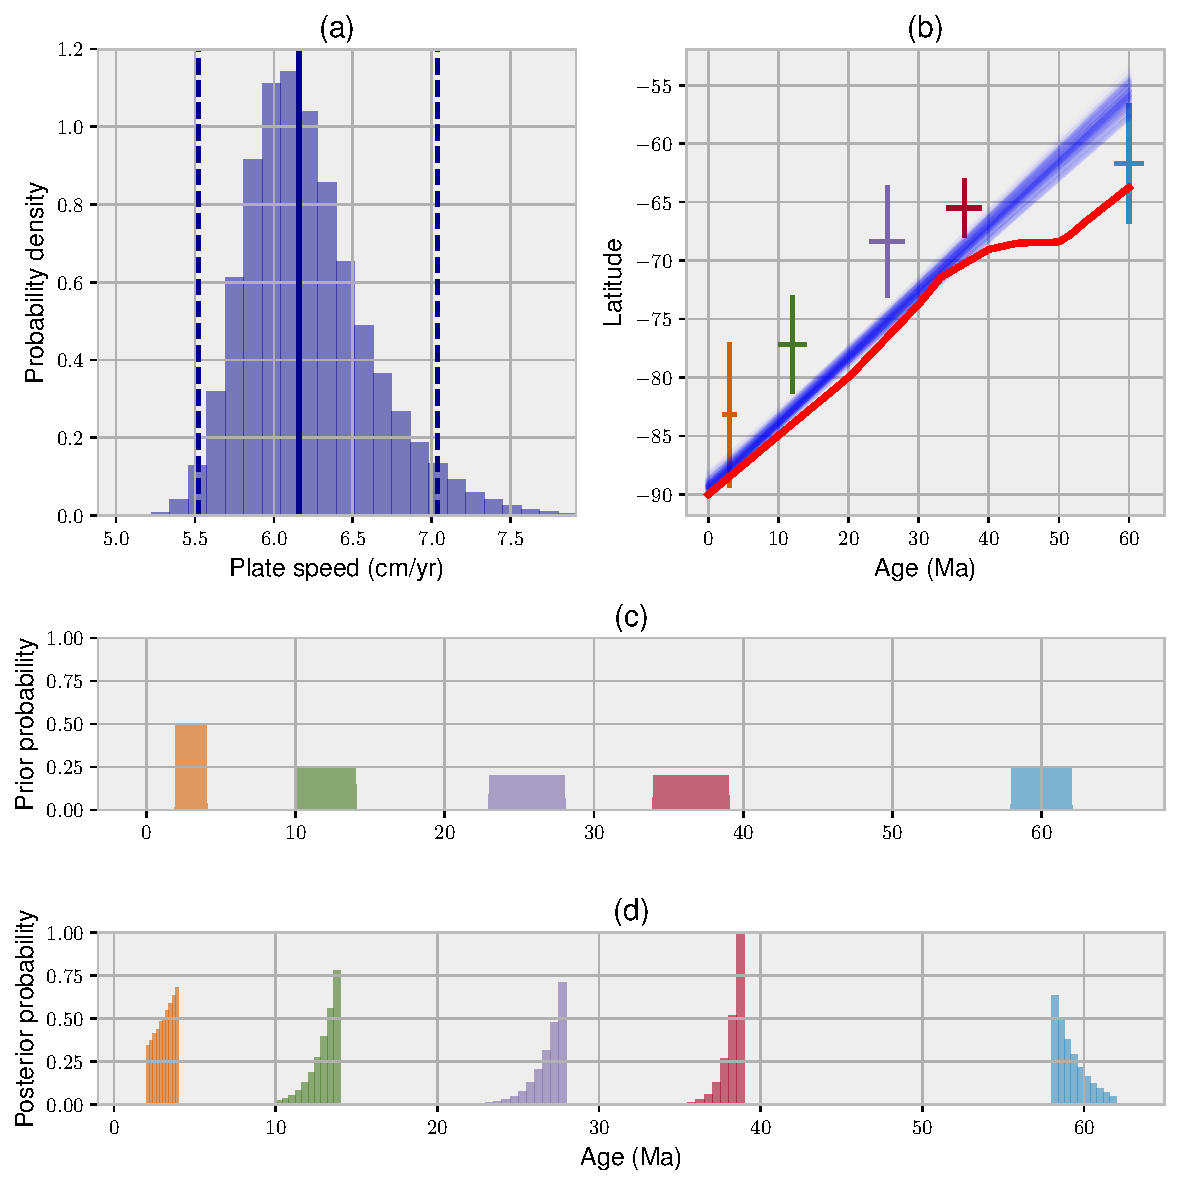
\includegraphics[width=0.9\textwidth]{figures/australia/australia_speeds_1.pdf}
\caption{}
\label{fig:australia_speeds_1}
\end{figure*}
\begin{figure*}
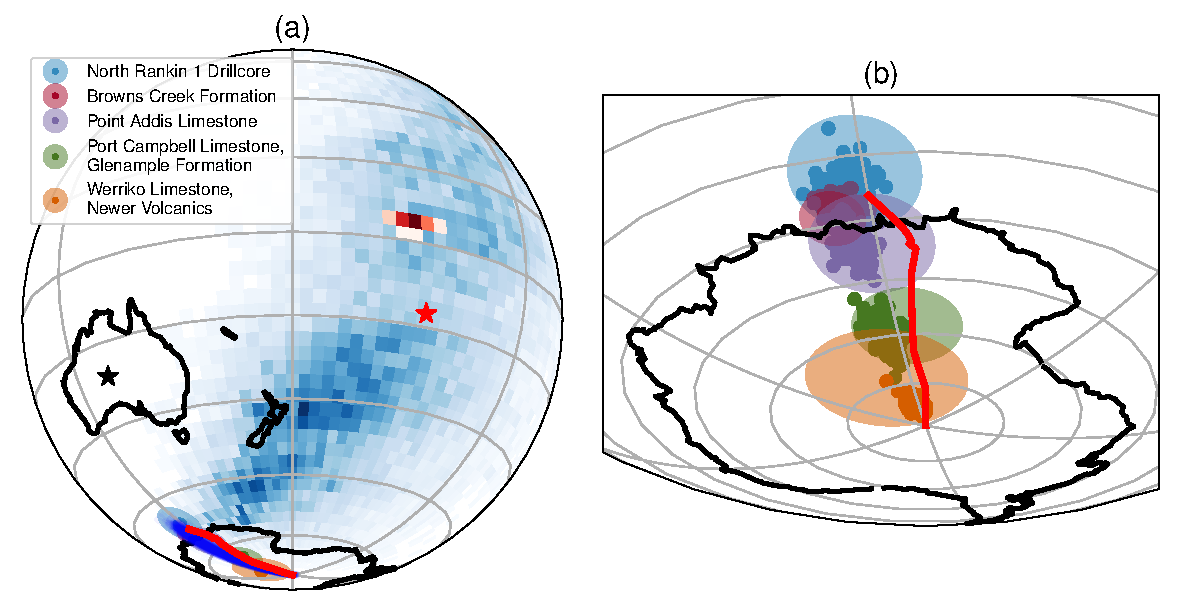
\includegraphics[width=0.9\textwidth]{figures/australia/australia_paths_2.pdf}
\caption{}
\label{fig:australia_paths_2}
\end{figure*}
\begin{figure*}
\includegraphics[width=0.9\textwidth]{figures/australia/australia_ages_2.pdf}
\caption{}
\label{fig:australia_ages_2}
\end{figure*}
\begin{figure*}
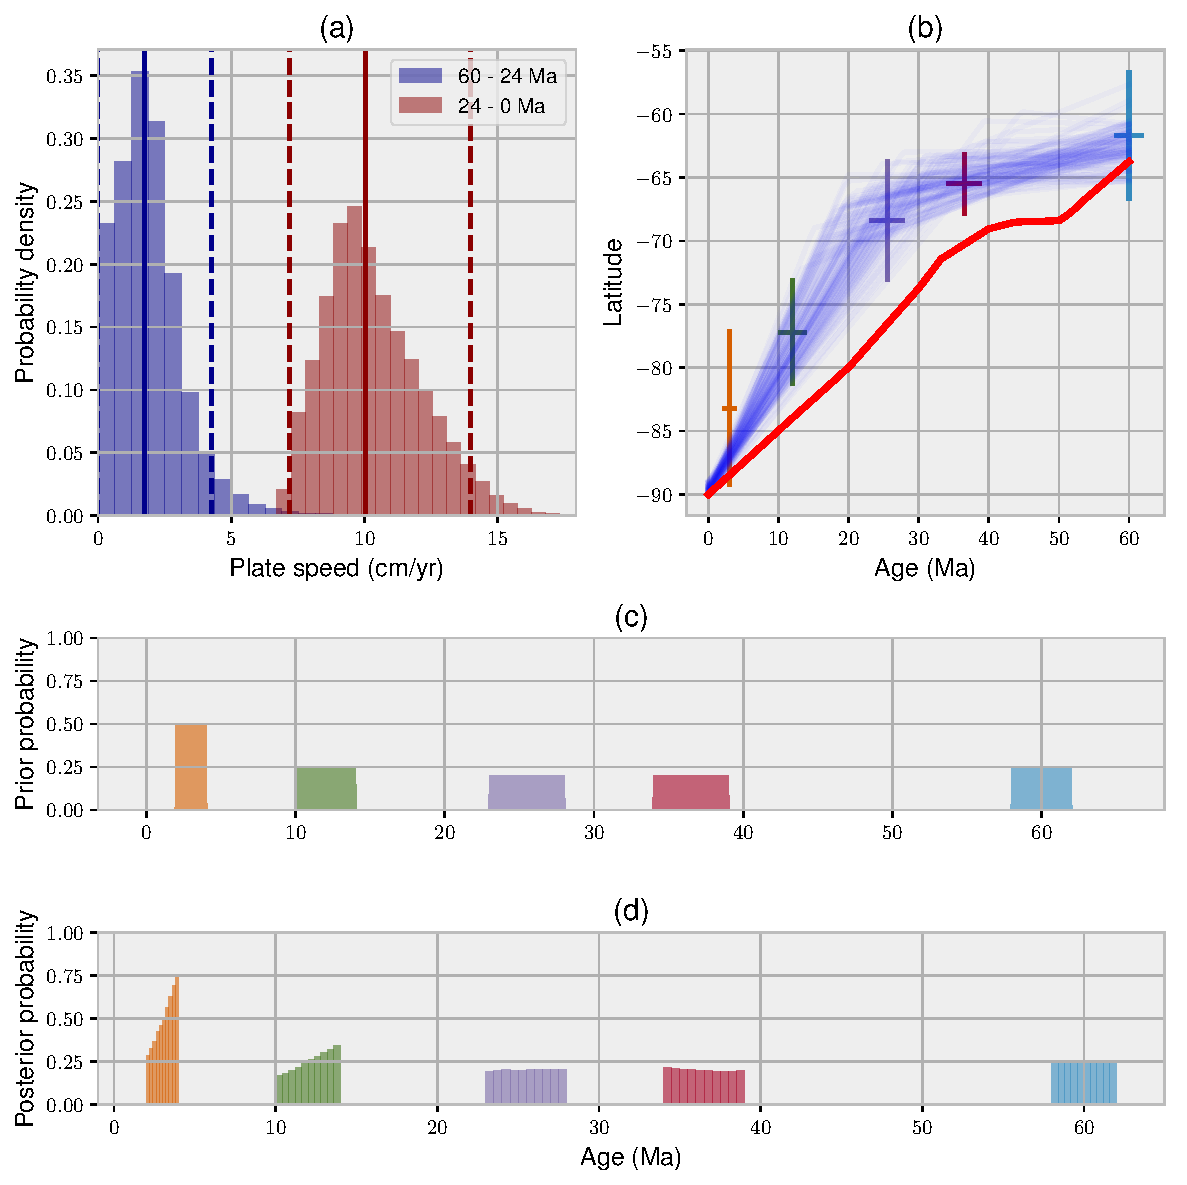
\includegraphics[width=0.9\textwidth]{figures/australia/australia_speeds_2.pdf}
\caption{}
\label{fig:australia_speeds_2}
\end{figure*}
\begin{figure*}
\includegraphics[width=0.9\textwidth]{figures/australia/australia_latitude_2.pdf}
\caption{}
\label{fig:australia_latitude_2}
\end{figure*}


\section{Application to the Keweenawan province}
\label{sec:keweenawan}
\subsection{Geologic context}
\citet{swanson2009no}
\subsection{Inversion for paleomagnetic Euler poles}
\clearpage

\begin{landscape}
\begin{tabular}{p{3cm} p{0.8cm} p{0.8cm} p{0.8cm} p{4cm} p{2.0cm} p{1.2cm} p{1.2cm} p{4.0cm}}
\toprule
                                     Pole &  $\psi_p$ &  $\phi_p$ &  $A_{95}$ &                                             Pole reference &            Age (Ma) & Lower age (Ma) & Upper age (Ma) &                                   Age reference \\
\midrule
                    Osler reverse (lower) &      40.9 &     218.6 &       4.8 &                            \citet{swanson2014confirmation} &                     &        1105.15 &           1110 &                          \citet{swanson2016new} \\
                    Osler reverse (upper) &      42.5 &     201.6 &       3.7 &     \citet{swanson2014confirmation,halls1974paleomagnetic} &  $1105.15 \pm 0.33$ &                &                &                          \citet{swanson2016new} \\
                Mamainse lower reversed 1 &      49.5 &     227.0 &       5.3 &                 \citet{swanson2009no, swanson2014magmatic} &                     &           1106 &           1112 &                     \citet{swanson2014magmatic} \\
                Mamainse lower reversed 2 &      37.5 &     205.2 &       4.5 &                 \citet{swanson2009no, swanson2014magmatic} &                     &           1102 &           1108 &                     \citet{swanson2014magmatic} \\
 Mamainse lower normal and upper reversed &      36.1 &     189.7 &       4.9 &                 \citet{swanson2009no, swanson2014magmatic} &  $1100.36 \pm 0.25$ &                &                &                     \citet{swanson2014magmatic} \\
                    Mamainse upper normal &      31.2 &     183.2 &       2.5 &                 \citet{swanson2009no, swanson2014magmatic} &                     &           1092 &           1098 &                     \citet{swanson2014magmatic} \\
                    Grand Portage Basalts &      46.6 &     201.5 &       6.8 &      \citet{books1968magnetization, tauxe2009paleosecular} &                     &        1105.28 &           1108 &                          \citet{swanson2016new} \\
               North Shore Volcanic Group &      35.8 &     182.1 &       3.1 &                              \citet{tauxe2009paleosecular} &                     &         1094.2 &         1095.8 &  \citet{schoene2006reassessing, swanson2016new} \\
                   Portage Lake Volcanics &      25.6 &     185.9 &       2.9 &           \citet{books1972paleomagnetism, hnat2006primary} &                     &        1091.67 &        1093.36 &                          \citet{swanson2016new} \\
                 Schroeder Lutsen Basalts &      27.1 &     187.8 &       3.0 &            \citet{tauxe2009paleosecular, fairchild2016end} &                     &           1085 &         1091.5 &                        \citet{fairchild2016end} \\
                         Lake Shore Traps &      23.1 &     186.4 &       4.0 &  \citet{diehl1994paleomagnetic, kulakov2013paleomagnetism} &                     &           1084 &           1091 &                        \citet{fairchild2016end} \\
            Michipicoten Island Formation &      17.0 &     174.7 &       4.4 &         \citet{palmer1987paleomagnetism, fairchild2016end} &    $1083.9 \pm 0.4$ &                &                &                        \citet{fairchild2016end} \\
                                    Freda &       2.2 &     179.0 &       4.2 &                            \citet{henry1977paleomagnetism} &                     &           1070 &         1085.5 &                        \citet{fairchild2016end} \\
\bottomrule
\end{tabular}

\end{landscape}

We investigated inverting the Keweenawan APW track for one, two, and three paleomagnetic Euler poles.
Adding a third PEP did not improve the fit, and it left one Euler pole completely unconstrained.
We interpret this as meaning that three PEPs is unnecessary given the data, and therefore focus
on the results with one and two PEPs.
We therefore focus on the results with one and two PEPs.

The fit with a single PEP is shown in Figure~\ref{fig:keweenawan_paths_1}.
The posterior distribution of the position for the Euler pole is shown in in blue,
and a sampling of the small-circle paths generated from the posterior distribution are ploted over the paleomagnetic poles.
Figure~\ref{fig:keweenawan_ages_1} shows the prior and posterior distributions for the ages of the poles,
and Figure~\ref{fig:keweenawan_speeds_1} shows the posterior distribution of the plate speed for Laurentia,
calculated with respect to Duluth, MN.

The median plate speed for the one-Euler pole inversion is 26.5 cm/yr, with an HPD interval at 95\% of 23.0-30.5 cm/yr.

The fit with two PEPs is shown in Figure~\ref{fig:keweenawan_paths_2}.
The posterior distribution of the position for the first Euler pole is shown in blue,
and the posterior distribution of the position for the second Euler pole is shown in red.
Figure~\ref{fig:keweenawan_ages_2} shows the prior and posterior distributions for the ages of the poles,
and Figure~\ref{fig:keweenawan_speeds_2} shows the posterior distribution of the plate speeds for the two rotations.

The inversion places the changepoint between the two Euler rotations at roughly 1098 Ma.
Before the chaingepoint the inverted plate motion is much faster, with median at 30 cm/yr
and an HPD at 95\% of 22.6-38.5 cm/yr. After the changepoint the plate motion has a median
of 13.7 cm/yr with and HPD at 95\% of 10.0-22.4 cm/yr.

This slowdown in plate speed at approximately 1098 Ma is consistent with the conclusions of
\citet{davis1997geochronology} and \citet{swanson2009no}, though the speeds in our
model reflect overall plate speeds (rather than just latitudinal speeds) and naturally incorporate age uncertainties.

\begin{figure*}
\includegraphics[width=0.9\textwidth]{figures/keweenawan/keweenawan_paths_1.pdf}
\caption[Inversion of the Keweenawan track for a single Euler rotation]{Inversion of the Keweenawan track for a single Euler rotation. The posterior probability distribution is shown in blue, and a representative sample of the tracks generated by the inversion are drawn over the paleomagnetic poles. Also shown is the outline of Laurentia, with the location of Duluth drawn as a star.}
\label{fig:keweenawan_paths_1}
\end{figure*}
\begin{figure*}
\includegraphics[width=0.9\textwidth]{figures/keweenawan/keweenawan_ages_1.pdf}
\caption[Age probability distributions for the single-Euler pole Keweenawan track inversion]{Age probability distributions for the single-Euler pole Keweenawn track inversion. Top: prior probability distribitions. Poles with radiometric ages are given Gaussian priors. Poles with stratigraphic age control are given uniform priors between their bracketing ages. Bottom: posterior probability distributions.}
\label{fig:keweenawan_ages_1}
\end{figure*}
\begin{figure*}
\includegraphics[width=0.9\textwidth]{figures/keweenawan/keweenawan_speeds_1.pdf}
\caption[Laurentian plate speed distribution for a single-Euler pole inversion]{Laurentian plate speed distribution for a single-Euler pole inversion.}
\label{fig:keweenawan_speeds_1}
\end{figure*}
\begin{figure*}
\includegraphics[width=0.9\textwidth]{figures/keweenawan/keweenawan_paths_2.pdf}
\caption[Inversion of the Keweenawan track for two Euler rotations]{Inversion of the Keweenawan track for a single Euler rotation. The posterior probability distribution is shown in blue, and a representative sample of the tracks generated by the inversion are drawn over the paleomagnetic poles. Also shown is the outline of Laurentia, with the location of Duluth drawn as a star.}
\label{fig:keweenawan_paths_2}
\end{figure*}
\begin{figure*}
\includegraphics[width=0.9\textwidth]{figures/keweenawan/keweenawan_ages_2.pdf}
\caption[Age probability distributions for the two-Euler pole Keweenawan track inversion]{Age probability distributions for the two-Euler pole Keweenawn track inversion. Top: prior probability distribitions. Poles with radiometric ages are given Gaussian priors. Poles with stratigraphic age control are given uniform priors between their bracketing ages. Bottom: posterior probability distributions.}
\label{fig:keweenawan_ages_2}
\end{figure*}
\begin{figure*}
\includegraphics[width=0.9\textwidth]{figures/keweenawan/keweenawan_speeds_2.pdf}
\caption[Laurentian plate speed distribution for a two-Euler pole inversion]{Laurentian plate speed distribution for a two-Euler pole inversion. The blue distribution shows the plate speeds for the first rotation, which occurs from approximately 1109-1098 Ma. The red distribution shows the plate speeds for the second rotation, which occurs from approximately 1098-1080 Ma. The changepoint is approximate, since it is also a random variable with its own posterior distribution. This inversion prefers a fast first rotation and a slower second rotation, though there is some overlap of the distributions.}
\label{fig:keweenawan_speeds_2}
\end{figure*}
\subsection{Plate speeds for Mesoproterozoic Laurentia}

\section{Conclusions}
\label{sec:conclusions}



%% The Appendices part is started with the command \appendix;
%% appendix sections are then done as normal sections
%% \appendix

%% \section{}
%% \label{}

%% If you have bibdatabase file and want bibtex to generate the
%% bibitems, please use
%%
\bibliographystyle{elsarticle-harv} 
\bibliography{bayesian_plate_reconstruction}

%% else use the following coding to input the bibitems directly in the
%% TeX file.

\end{document}

\endinput
%%
%% End of file `elsarticle-template-harv.tex'.
